\makeatletter
\def\input@path{{../}}
\makeatother

\documentclass[../preambulo.tex]{subfiles}


\begin{document}

\section{Segunda sección}


Vestibulum ut dui ipsum. Integer euismod euismod mauris a facilisis. Vivamus commodo nibh libero, semper gravida tellus vulputate sit amet. Quisque ut fermentum mi. Etiam efficitur euismod turpis. Suspendisse potenti. Suspendisse non bibendum ipsum, consequat lacinia tellus. Sed rhoncus tincidunt orci quis consectetur. Maecenas quis rhoncus risus. Ut arcu risus, varius sit amet magna quis, imperdiet aliquet erat.


% Aquí estamos definiendo un elemento deslizante que contiene una imagen.
\begin{figure}[H]
	\centering
	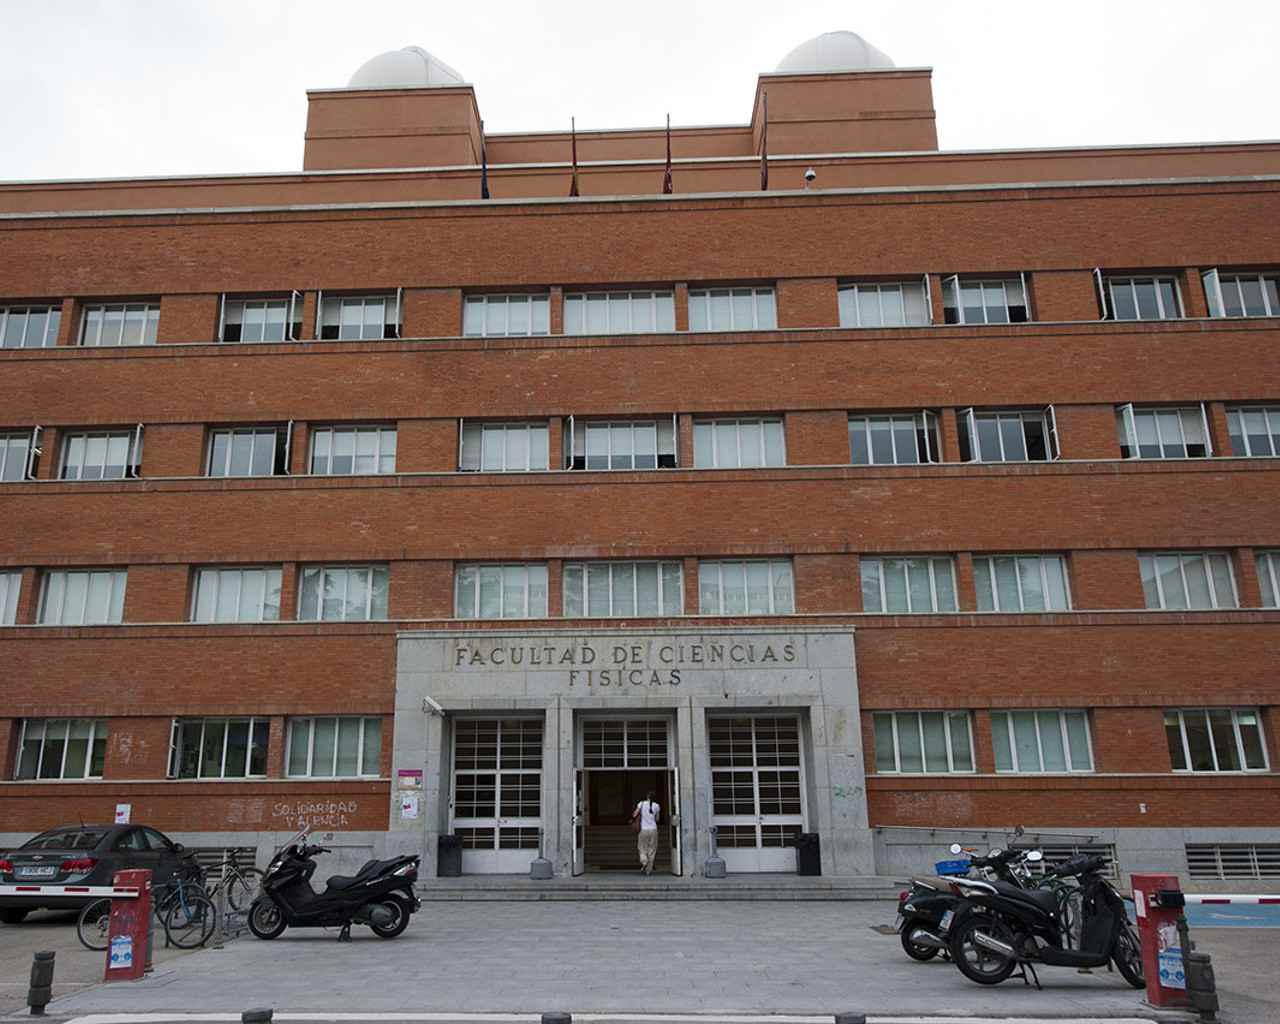
\includegraphics[scale=.3]{img/imagen}	% No he añadido
	\caption{Una fotografía de la entrada de la Facultad de Ciencias Físicas de la UCM.}
	\label{fig:patio}
\end{figure}



Ut nec purus aliquam metus auctor malesuada eget et massa. Donec nec est eleifend, sagittis enim et, pharetra magna. Aenean facilisis augue vitae arcu condimentum, sit amet aliquet erat ullamcorper. Sed ornare risus sit amet lacinia ultricies. Sed id hendrerit metus, eget interdum felis. Interdum et malesuada fames ac ante ipsum primis in faucibus. Pellentesque facilisis sodales nunc sit amet euismod. Donec interdum ut neque ut pretium. Sed vel sodales quam.

% En este párrafo hemos hecho una referencia a la primera sección.
Referencia a la sección \ref{Sec:inicio}.



% Aquí hemos definido una sección que no se indexará ni se numerará.
\section*{Modo matemático}


Fusce porta velit imperdiet elit interdum, ac bibendum purus porta. Nunc ante odio, faucibus sed tincidunt vulputate, egestas aliquet felis. Sed mollis condimentum ex, sit amet consequat elit tempus non. Suspendisse a nunc in massa bibendum tempor. Morbi elementum quam libero, vitae euismod massa volutpat at.

% Esto es una ecuación "en línea".
Suspendisse non arcu $\sum_i ^n x_i$ sit amet mauris tempus lobortis et sit amet sapien. 

% Aquí va una ecuación "destacada". Nótese que está numerada.
\begin{equation}
	E = mc^2
\end{equation}


% Esto es un ejemplo de una ecuación "destacada" sin numerar.
\[
	\nabla \cdot %
	\vec{ B } = 0
\]



\subsection*{Tipografía en modo matemático}


Fusce porta velit imperdiet elit interdum, ac bibendum purus porta. Nunc ante odio, faucibus sed tincidunt vulputate, egestas aliquet felis. Sed mollis condimentum ex, sit amet consequat elit tempus non. Suspendisse a nunc in massa bibendum tempor. Morbi elementum quam libero, vitae euismod massa volutpat at. Suspendisse non arcu $\sum_i ^n x_i$ sit amet mauris tempus lobortis et sit amet sapien. 


% Aquí tenemos algunos ejemplos de la tipografía y espacios que pueden usarse en el modo matemático.
\[
		\mathrm{tipografia\ recta}
\]

\[
		\mathit{tipografia\ \ cursiva}
\]

\[
		\mathbf{tipografia\quad negrita}
\]

\[
		tipografia\qquad negrita de pizarra
\]

\[
		\int \int \mathrm{d} x
\]

\[
		\derivada{2}{f}{x}
\]

\[
		\int \! \! \! \int \mathrm{d} x
\]

\[
		\iint \dif x
\]



\end{document}